% yaml_workflow.tex
% TikZ diagram for Stata Journal article: YAML-enabled cross-platform workflow
% Author: João Pedro Azevedo
% Date: December 2025
%
% Usage: Include in main document with:
%   % yaml_workflow.tex
% TikZ diagram for Stata Journal article: YAML-enabled cross-platform workflow
% Author: João Pedro Azevedo
% Date: December 2025
%
% Usage: Include in main document with:
%   % yaml_workflow.tex
% TikZ diagram for Stata Journal article: YAML-enabled cross-platform workflow
% Author: João Pedro Azevedo
% Date: December 2025
%
% Usage: Include in main document with:
%   % yaml_workflow.tex
% TikZ diagram for Stata Journal article: YAML-enabled cross-platform workflow
% Author: João Pedro Azevedo
% Date: December 2025
%
% Usage: Include in main document with:
%   \input{figures/yaml_workflow.tex}
%
% Or compile standalone:
%   pdflatex yaml_workflow.tex

\documentclass[tikz,border=10pt]{standalone}
\usepackage{tikz}
\usetikzlibrary{shapes.geometric, arrows.meta, positioning, fit, backgrounds, calc}

\begin{document}

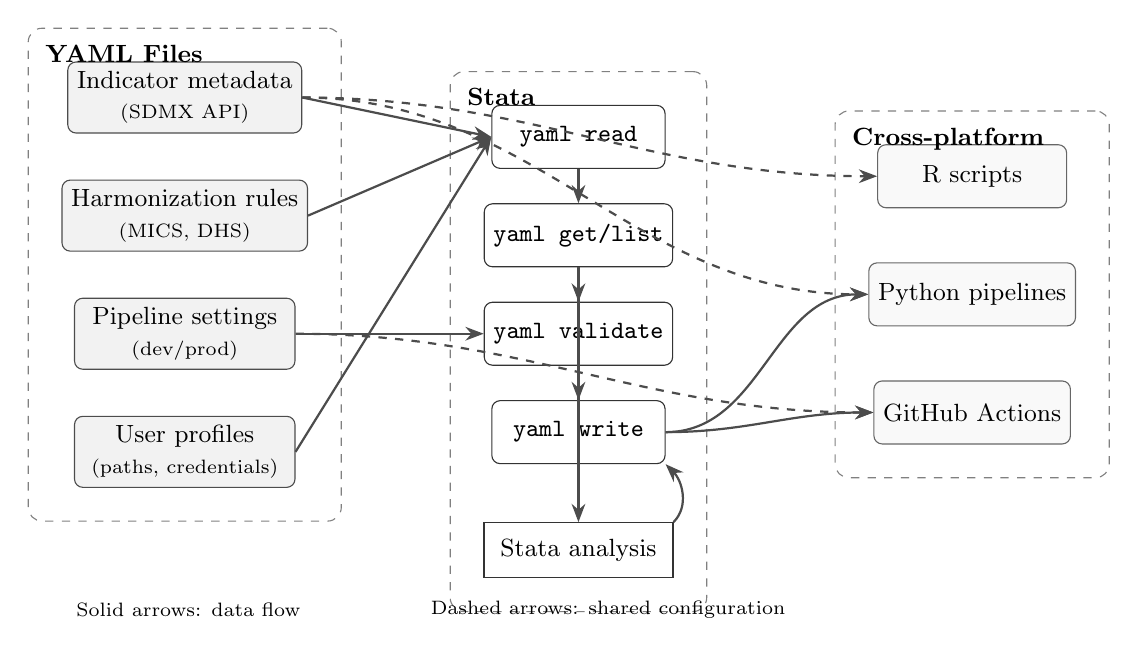
\begin{tikzpicture}[
    % Node styles
    yamlbox/.style={
        rectangle, 
        rounded corners=3pt,
        draw=black!70, 
        fill=gray!10,
        minimum width=2.8cm, 
        minimum height=0.9cm,
        font=\small,
        align=center
    },
    statabox/.style={
        rectangle, 
        rounded corners=3pt,
        draw=black!80, 
        fill=white,
        minimum width=2.2cm, 
        minimum height=0.8cm,
        font=\small\ttfamily
    },
    otherbox/.style={
        rectangle, 
        rounded corners=3pt,
        draw=black!60, 
        fill=gray!5,
        minimum width=2.4cm, 
        minimum height=0.8cm,
        font=\small
    },
    groupbox/.style={
        rectangle,
        rounded corners=5pt,
        draw=black!50,
        dashed,
        inner sep=8pt
    },
    grouplabel/.style={
        font=\small\bfseries,
        anchor=north west
    },
    arrow/.style={
        ->,
        >=Stealth,
        thick,
        black!70
    },
    biarrow/.style={
        <->,
        >=Stealth,
        thick,
        black!70
    }
]

% === YAML Configuration Files (Left) ===
\node[yamlbox] (yaml1) at (0, 3) {Indicator metadata\\{\scriptsize(SDMX API)}};
\node[yamlbox] (yaml2) at (0, 1.5) {Harmonization rules\\{\scriptsize(MICS, DHS)}};
\node[yamlbox] (yaml3) at (0, 0) {Pipeline settings\\{\scriptsize(dev/prod)}};
\node[yamlbox] (yaml4) at (0, -1.5) {User profiles\\{\scriptsize(paths, credentials)}};

% Group box for YAML
\begin{scope}[on background layer]
    \node[groupbox, fit=(yaml1)(yaml2)(yaml3)(yaml4), inner sep=12pt] (yamlgroup) {};
\end{scope}
\node[grouplabel] at ($(yamlgroup.north west) + (0.1, -0.1)$) {YAML Files};

% === Stata Commands (Center) ===
\node[statabox] (read) at (5, 2.5) {yaml read};
\node[statabox] (get) at (5, 1.25) {yaml get/list};
\node[statabox] (validate) at (5, 0) {yaml validate};
\node[statabox] (write) at (5, -1.25) {yaml write};

% Stata processing node
\node[rectangle, draw=black!80, fill=white, minimum width=2.4cm, minimum height=0.7cm, font=\small] 
    (process) at (5, -2.75) {Stata analysis};

% Group box for Stata
\begin{scope}[on background layer]
    \node[groupbox, fit=(read)(get)(validate)(write)(process), inner sep=12pt] (statagroup) {};
\end{scope}
\node[grouplabel] at ($(statagroup.north west) + (0.1, -0.1)$) {Stata};

% === Other Tools (Right) ===
\node[otherbox] (r) at (10, 2) {R scripts};
\node[otherbox] (python) at (10, 0.5) {Python pipelines};
\node[otherbox] (github) at (10, -1) {GitHub Actions};

% Group box for Other Tools
\begin{scope}[on background layer]
    \node[groupbox, fit=(r)(python)(github), inner sep=12pt] (othergroup) {};
\end{scope}
\node[grouplabel] at ($(othergroup.north west) + (0.1, -0.1)$) {Cross-platform};

% === Arrows: YAML to Stata ===
\draw[arrow] (yaml1.east) -- (read.west);
\draw[arrow] (yaml2.east) -- (read.west);
\draw[arrow] (yaml3.east) -- (validate.west);
\draw[arrow] (yaml4.east) -- (read.west);

% === Arrows: Within Stata ===
\draw[arrow] (read) -- (get);
\draw[arrow] (get) -- (validate);
\draw[arrow] (validate) -- (write);
\draw[arrow] (get.south) to[out=-90, in=90] (process.north);
\draw[arrow] (process.north east) to[out=45, in=-45] (write.south east);

% === Arrows: YAML to Other Tools (shared config) ===
\draw[arrow, dashed] (yaml1.east) to[out=0, in=180] (r.west);
\draw[arrow, dashed] (yaml1.east) to[out=0, in=180] (python.west);
\draw[arrow, dashed] (yaml3.east) to[out=0, in=180] (github.west);

% === Arrows: Stata to Other Tools ===
\draw[arrow] (write.east) to[out=0, in=180] (python.west);
\draw[arrow] (write.east) to[out=0, in=180] (github.west);

% === Legend ===
\node[font=\scriptsize, anchor=west] at (-1.5, -3.5) {Solid arrows: data flow};
\node[font=\scriptsize, anchor=west] at (3, -3.5) {Dashed arrows: shared configuration};

\end{tikzpicture}

\end{document}

%
% Or compile standalone:
%   pdflatex yaml_workflow.tex

\documentclass[tikz,border=10pt]{standalone}
\usepackage{tikz}
\usetikzlibrary{shapes.geometric, arrows.meta, positioning, fit, backgrounds, calc}

\begin{document}

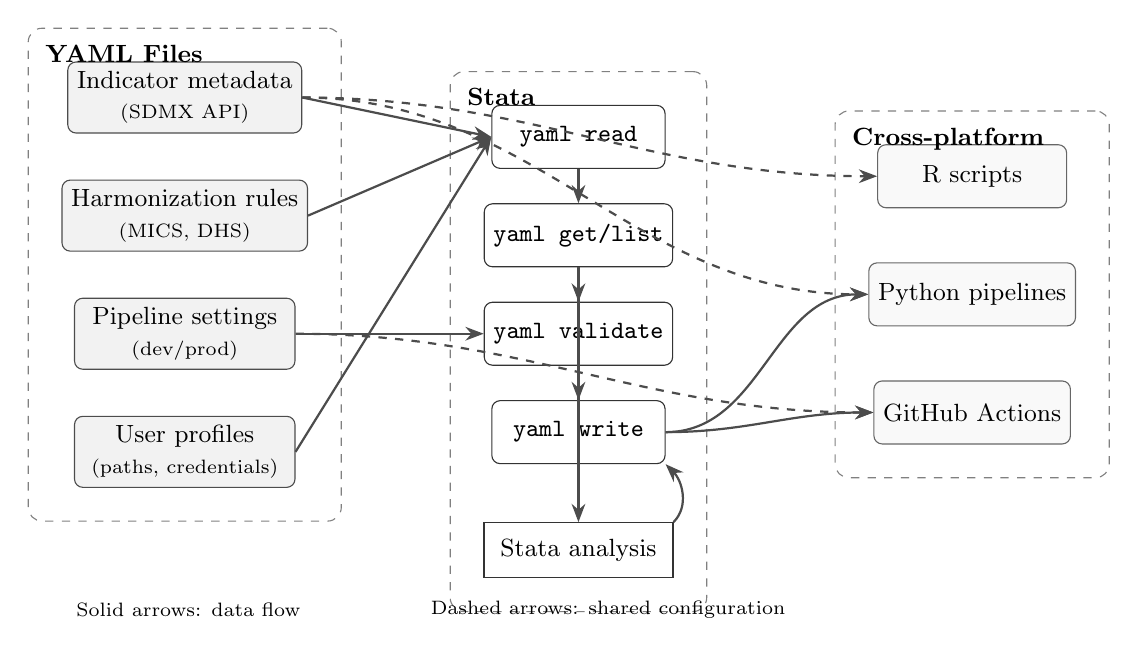
\begin{tikzpicture}[
    % Node styles
    yamlbox/.style={
        rectangle, 
        rounded corners=3pt,
        draw=black!70, 
        fill=gray!10,
        minimum width=2.8cm, 
        minimum height=0.9cm,
        font=\small,
        align=center
    },
    statabox/.style={
        rectangle, 
        rounded corners=3pt,
        draw=black!80, 
        fill=white,
        minimum width=2.2cm, 
        minimum height=0.8cm,
        font=\small\ttfamily
    },
    otherbox/.style={
        rectangle, 
        rounded corners=3pt,
        draw=black!60, 
        fill=gray!5,
        minimum width=2.4cm, 
        minimum height=0.8cm,
        font=\small
    },
    groupbox/.style={
        rectangle,
        rounded corners=5pt,
        draw=black!50,
        dashed,
        inner sep=8pt
    },
    grouplabel/.style={
        font=\small\bfseries,
        anchor=north west
    },
    arrow/.style={
        ->,
        >=Stealth,
        thick,
        black!70
    },
    biarrow/.style={
        <->,
        >=Stealth,
        thick,
        black!70
    }
]

% === YAML Configuration Files (Left) ===
\node[yamlbox] (yaml1) at (0, 3) {Indicator metadata\\{\scriptsize(SDMX API)}};
\node[yamlbox] (yaml2) at (0, 1.5) {Harmonization rules\\{\scriptsize(MICS, DHS)}};
\node[yamlbox] (yaml3) at (0, 0) {Pipeline settings\\{\scriptsize(dev/prod)}};
\node[yamlbox] (yaml4) at (0, -1.5) {User profiles\\{\scriptsize(paths, credentials)}};

% Group box for YAML
\begin{scope}[on background layer]
    \node[groupbox, fit=(yaml1)(yaml2)(yaml3)(yaml4), inner sep=12pt] (yamlgroup) {};
\end{scope}
\node[grouplabel] at ($(yamlgroup.north west) + (0.1, -0.1)$) {YAML Files};

% === Stata Commands (Center) ===
\node[statabox] (read) at (5, 2.5) {yaml read};
\node[statabox] (get) at (5, 1.25) {yaml get/list};
\node[statabox] (validate) at (5, 0) {yaml validate};
\node[statabox] (write) at (5, -1.25) {yaml write};

% Stata processing node
\node[rectangle, draw=black!80, fill=white, minimum width=2.4cm, minimum height=0.7cm, font=\small] 
    (process) at (5, -2.75) {Stata analysis};

% Group box for Stata
\begin{scope}[on background layer]
    \node[groupbox, fit=(read)(get)(validate)(write)(process), inner sep=12pt] (statagroup) {};
\end{scope}
\node[grouplabel] at ($(statagroup.north west) + (0.1, -0.1)$) {Stata};

% === Other Tools (Right) ===
\node[otherbox] (r) at (10, 2) {R scripts};
\node[otherbox] (python) at (10, 0.5) {Python pipelines};
\node[otherbox] (github) at (10, -1) {GitHub Actions};

% Group box for Other Tools
\begin{scope}[on background layer]
    \node[groupbox, fit=(r)(python)(github), inner sep=12pt] (othergroup) {};
\end{scope}
\node[grouplabel] at ($(othergroup.north west) + (0.1, -0.1)$) {Cross-platform};

% === Arrows: YAML to Stata ===
\draw[arrow] (yaml1.east) -- (read.west);
\draw[arrow] (yaml2.east) -- (read.west);
\draw[arrow] (yaml3.east) -- (validate.west);
\draw[arrow] (yaml4.east) -- (read.west);

% === Arrows: Within Stata ===
\draw[arrow] (read) -- (get);
\draw[arrow] (get) -- (validate);
\draw[arrow] (validate) -- (write);
\draw[arrow] (get.south) to[out=-90, in=90] (process.north);
\draw[arrow] (process.north east) to[out=45, in=-45] (write.south east);

% === Arrows: YAML to Other Tools (shared config) ===
\draw[arrow, dashed] (yaml1.east) to[out=0, in=180] (r.west);
\draw[arrow, dashed] (yaml1.east) to[out=0, in=180] (python.west);
\draw[arrow, dashed] (yaml3.east) to[out=0, in=180] (github.west);

% === Arrows: Stata to Other Tools ===
\draw[arrow] (write.east) to[out=0, in=180] (python.west);
\draw[arrow] (write.east) to[out=0, in=180] (github.west);

% === Legend ===
\node[font=\scriptsize, anchor=west] at (-1.5, -3.5) {Solid arrows: data flow};
\node[font=\scriptsize, anchor=west] at (3, -3.5) {Dashed arrows: shared configuration};

\end{tikzpicture}

\end{document}

%
% Or compile standalone:
%   pdflatex yaml_workflow.tex

\documentclass[tikz,border=10pt]{standalone}
\usepackage{tikz}
\usetikzlibrary{shapes.geometric, arrows.meta, positioning, fit, backgrounds, calc}

\begin{document}

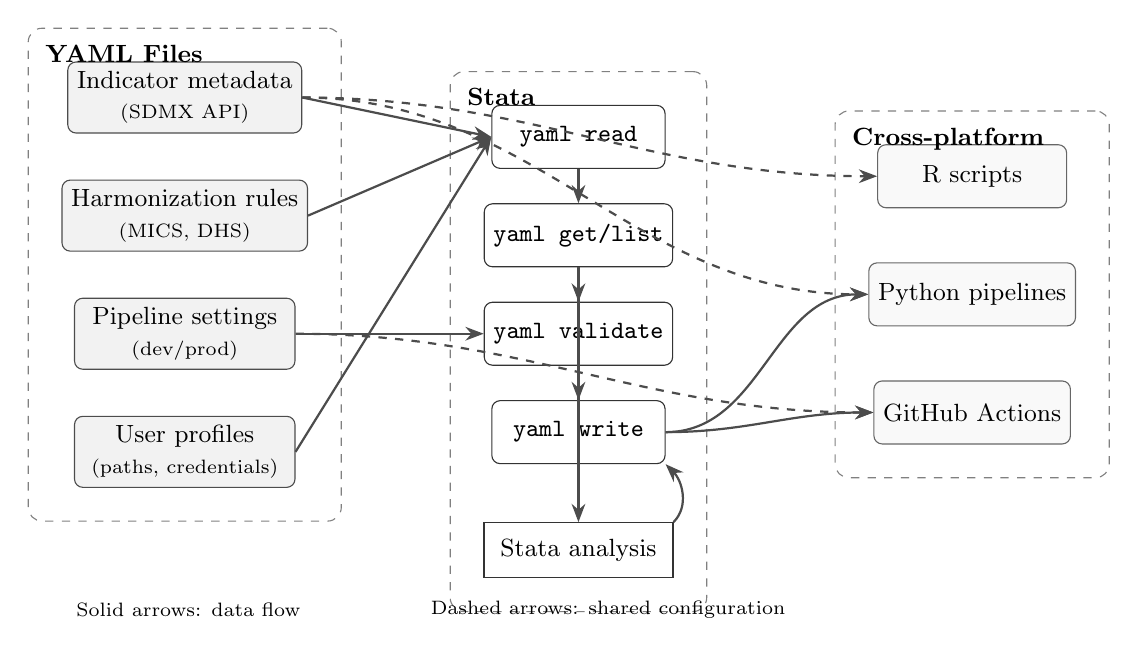
\begin{tikzpicture}[
    % Node styles
    yamlbox/.style={
        rectangle, 
        rounded corners=3pt,
        draw=black!70, 
        fill=gray!10,
        minimum width=2.8cm, 
        minimum height=0.9cm,
        font=\small,
        align=center
    },
    statabox/.style={
        rectangle, 
        rounded corners=3pt,
        draw=black!80, 
        fill=white,
        minimum width=2.2cm, 
        minimum height=0.8cm,
        font=\small\ttfamily
    },
    otherbox/.style={
        rectangle, 
        rounded corners=3pt,
        draw=black!60, 
        fill=gray!5,
        minimum width=2.4cm, 
        minimum height=0.8cm,
        font=\small
    },
    groupbox/.style={
        rectangle,
        rounded corners=5pt,
        draw=black!50,
        dashed,
        inner sep=8pt
    },
    grouplabel/.style={
        font=\small\bfseries,
        anchor=north west
    },
    arrow/.style={
        ->,
        >=Stealth,
        thick,
        black!70
    },
    biarrow/.style={
        <->,
        >=Stealth,
        thick,
        black!70
    }
]

% === YAML Configuration Files (Left) ===
\node[yamlbox] (yaml1) at (0, 3) {Indicator metadata\\{\scriptsize(SDMX API)}};
\node[yamlbox] (yaml2) at (0, 1.5) {Harmonization rules\\{\scriptsize(MICS, DHS)}};
\node[yamlbox] (yaml3) at (0, 0) {Pipeline settings\\{\scriptsize(dev/prod)}};
\node[yamlbox] (yaml4) at (0, -1.5) {User profiles\\{\scriptsize(paths, credentials)}};

% Group box for YAML
\begin{scope}[on background layer]
    \node[groupbox, fit=(yaml1)(yaml2)(yaml3)(yaml4), inner sep=12pt] (yamlgroup) {};
\end{scope}
\node[grouplabel] at ($(yamlgroup.north west) + (0.1, -0.1)$) {YAML Files};

% === Stata Commands (Center) ===
\node[statabox] (read) at (5, 2.5) {yaml read};
\node[statabox] (get) at (5, 1.25) {yaml get/list};
\node[statabox] (validate) at (5, 0) {yaml validate};
\node[statabox] (write) at (5, -1.25) {yaml write};

% Stata processing node
\node[rectangle, draw=black!80, fill=white, minimum width=2.4cm, minimum height=0.7cm, font=\small] 
    (process) at (5, -2.75) {Stata analysis};

% Group box for Stata
\begin{scope}[on background layer]
    \node[groupbox, fit=(read)(get)(validate)(write)(process), inner sep=12pt] (statagroup) {};
\end{scope}
\node[grouplabel] at ($(statagroup.north west) + (0.1, -0.1)$) {Stata};

% === Other Tools (Right) ===
\node[otherbox] (r) at (10, 2) {R scripts};
\node[otherbox] (python) at (10, 0.5) {Python pipelines};
\node[otherbox] (github) at (10, -1) {GitHub Actions};

% Group box for Other Tools
\begin{scope}[on background layer]
    \node[groupbox, fit=(r)(python)(github), inner sep=12pt] (othergroup) {};
\end{scope}
\node[grouplabel] at ($(othergroup.north west) + (0.1, -0.1)$) {Cross-platform};

% === Arrows: YAML to Stata ===
\draw[arrow] (yaml1.east) -- (read.west);
\draw[arrow] (yaml2.east) -- (read.west);
\draw[arrow] (yaml3.east) -- (validate.west);
\draw[arrow] (yaml4.east) -- (read.west);

% === Arrows: Within Stata ===
\draw[arrow] (read) -- (get);
\draw[arrow] (get) -- (validate);
\draw[arrow] (validate) -- (write);
\draw[arrow] (get.south) to[out=-90, in=90] (process.north);
\draw[arrow] (process.north east) to[out=45, in=-45] (write.south east);

% === Arrows: YAML to Other Tools (shared config) ===
\draw[arrow, dashed] (yaml1.east) to[out=0, in=180] (r.west);
\draw[arrow, dashed] (yaml1.east) to[out=0, in=180] (python.west);
\draw[arrow, dashed] (yaml3.east) to[out=0, in=180] (github.west);

% === Arrows: Stata to Other Tools ===
\draw[arrow] (write.east) to[out=0, in=180] (python.west);
\draw[arrow] (write.east) to[out=0, in=180] (github.west);

% === Legend ===
\node[font=\scriptsize, anchor=west] at (-1.5, -3.5) {Solid arrows: data flow};
\node[font=\scriptsize, anchor=west] at (3, -3.5) {Dashed arrows: shared configuration};

\end{tikzpicture}

\end{document}

%
% Or compile standalone:
%   pdflatex yaml_workflow.tex

\documentclass[tikz,border=10pt]{standalone}
\usepackage{tikz}
\usetikzlibrary{shapes.geometric, arrows.meta, positioning, fit, backgrounds, calc}

\begin{document}

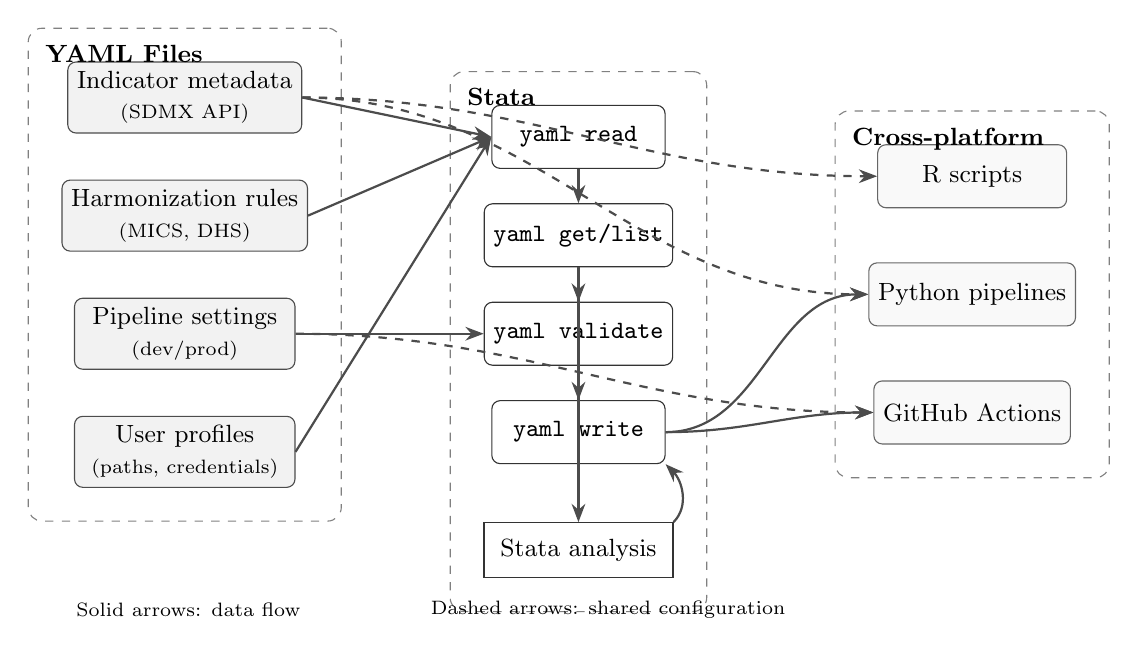
\begin{tikzpicture}[
    % Node styles
    yamlbox/.style={
        rectangle, 
        rounded corners=3pt,
        draw=black!70, 
        fill=gray!10,
        minimum width=2.8cm, 
        minimum height=0.9cm,
        font=\small,
        align=center
    },
    statabox/.style={
        rectangle, 
        rounded corners=3pt,
        draw=black!80, 
        fill=white,
        minimum width=2.2cm, 
        minimum height=0.8cm,
        font=\small\ttfamily
    },
    otherbox/.style={
        rectangle, 
        rounded corners=3pt,
        draw=black!60, 
        fill=gray!5,
        minimum width=2.4cm, 
        minimum height=0.8cm,
        font=\small
    },
    groupbox/.style={
        rectangle,
        rounded corners=5pt,
        draw=black!50,
        dashed,
        inner sep=8pt
    },
    grouplabel/.style={
        font=\small\bfseries,
        anchor=north west
    },
    arrow/.style={
        ->,
        >=Stealth,
        thick,
        black!70
    },
    biarrow/.style={
        <->,
        >=Stealth,
        thick,
        black!70
    }
]

% === YAML Configuration Files (Left) ===
\node[yamlbox] (yaml1) at (0, 3) {Indicator metadata\\{\scriptsize(SDMX API)}};
\node[yamlbox] (yaml2) at (0, 1.5) {Harmonization rules\\{\scriptsize(MICS, DHS)}};
\node[yamlbox] (yaml3) at (0, 0) {Pipeline settings\\{\scriptsize(dev/prod)}};
\node[yamlbox] (yaml4) at (0, -1.5) {User profiles\\{\scriptsize(paths, credentials)}};

% Group box for YAML
\begin{scope}[on background layer]
    \node[groupbox, fit=(yaml1)(yaml2)(yaml3)(yaml4), inner sep=12pt] (yamlgroup) {};
\end{scope}
\node[grouplabel] at ($(yamlgroup.north west) + (0.1, -0.1)$) {YAML Files};

% === Stata Commands (Center) ===
\node[statabox] (read) at (5, 2.5) {yaml read};
\node[statabox] (get) at (5, 1.25) {yaml get/list};
\node[statabox] (validate) at (5, 0) {yaml validate};
\node[statabox] (write) at (5, -1.25) {yaml write};

% Stata processing node
\node[rectangle, draw=black!80, fill=white, minimum width=2.4cm, minimum height=0.7cm, font=\small] 
    (process) at (5, -2.75) {Stata analysis};

% Group box for Stata
\begin{scope}[on background layer]
    \node[groupbox, fit=(read)(get)(validate)(write)(process), inner sep=12pt] (statagroup) {};
\end{scope}
\node[grouplabel] at ($(statagroup.north west) + (0.1, -0.1)$) {Stata};

% === Other Tools (Right) ===
\node[otherbox] (r) at (10, 2) {R scripts};
\node[otherbox] (python) at (10, 0.5) {Python pipelines};
\node[otherbox] (github) at (10, -1) {GitHub Actions};

% Group box for Other Tools
\begin{scope}[on background layer]
    \node[groupbox, fit=(r)(python)(github), inner sep=12pt] (othergroup) {};
\end{scope}
\node[grouplabel] at ($(othergroup.north west) + (0.1, -0.1)$) {Cross-platform};

% === Arrows: YAML to Stata ===
\draw[arrow] (yaml1.east) -- (read.west);
\draw[arrow] (yaml2.east) -- (read.west);
\draw[arrow] (yaml3.east) -- (validate.west);
\draw[arrow] (yaml4.east) -- (read.west);

% === Arrows: Within Stata ===
\draw[arrow] (read) -- (get);
\draw[arrow] (get) -- (validate);
\draw[arrow] (validate) -- (write);
\draw[arrow] (get.south) to[out=-90, in=90] (process.north);
\draw[arrow] (process.north east) to[out=45, in=-45] (write.south east);

% === Arrows: YAML to Other Tools (shared config) ===
\draw[arrow, dashed] (yaml1.east) to[out=0, in=180] (r.west);
\draw[arrow, dashed] (yaml1.east) to[out=0, in=180] (python.west);
\draw[arrow, dashed] (yaml3.east) to[out=0, in=180] (github.west);

% === Arrows: Stata to Other Tools ===
\draw[arrow] (write.east) to[out=0, in=180] (python.west);
\draw[arrow] (write.east) to[out=0, in=180] (github.west);

% === Legend ===
\node[font=\scriptsize, anchor=west] at (-1.5, -3.5) {Solid arrows: data flow};
\node[font=\scriptsize, anchor=west] at (3, -3.5) {Dashed arrows: shared configuration};

\end{tikzpicture}

\end{document}
